\chapter{Background and Related Works}\label{ch2}
\noindent
In this chapter, we first present a few background concepts needed for developing the foundation of our proposed work. We 
also present an overview of different methods proposed in the literature of scheduling around DRAM.

\section{Background}\label{back}
\noindent
In this section, we discuss a few background concepts.

\subsection{Organization of DRAM}\label{b1}

\begin{figure}[t]
\centering
\fbox{
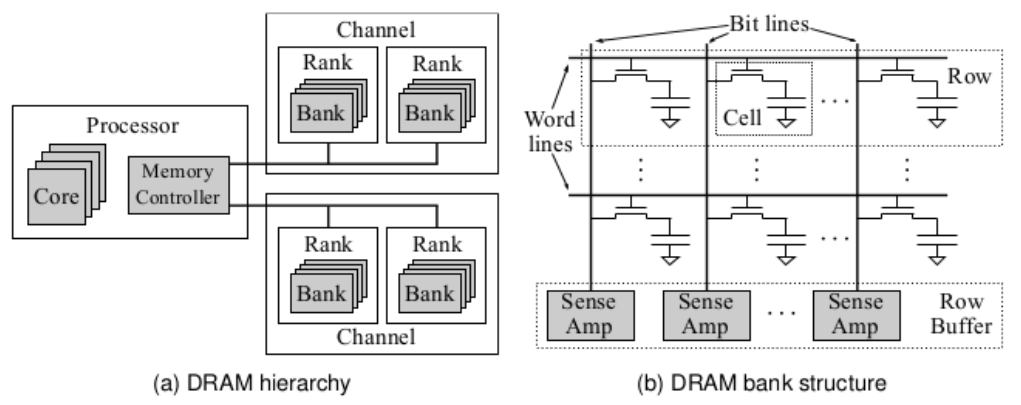
\includegraphics[width=12cm,height=7cm]{Dram_org.png}
}
\caption{Organisation of DRAM}
\label{fig3}
\end{figure}



\begin{figure}[t]
\centering
\fbox{
\includegraphics[width=8cm,height=5cm]{dram_state.png}
}
\caption{Simplified overview of important states of a DRAM}
\label{fig4}
\end{figure}


\noindent
Main memory is stored in DRAM cells that have much higher storage density. DRAM chips are large, rectangular arrays of memory 
cells with support logic that is used for reading and writing data in the arrays, and refresh circuitry to maintain the 
integrity of stored data~\cite{wiki:xxx1}. According to storage oraganization, memory is hierarchically organized into DIMM, 
rank, bank and array. DRAM devices are composed of basic blocks of DRAM memory. Multiple DRAM devices are accessed in parallel 
which together forms a DRAM rank~\cite{Rixner:2000:MAS:342001.339668}. DRAM devices in the same rank share same bus for 
address and command and another bus for data communication. Each DRAM device is made up of multiple DRAM arrays which store 
the data. Each of these arrays can be accessed independently. A group of DRAM arrays in different DRAM devices that are 
accessed together forms a DRAM bank. A DRAM bank is a 2D array of cells: rows x columns. A DRAM row is also called a DRAM 
page. Memory arrays are arranged in rows and columns of memory cells called wordlines and bitlines, respectively. Each memory 
cell has a unique location or address defined by the intersection of a row and a column. A DRAM cell stores a bit in a 
capacitor and hence they are needed to be charged periodically to prevent loss of data. Fig.\ref{fig3} shows the 
organisation of DRAM.

\subsection{DRAM access commands}\label{b2}
\noindent
A number of DRAM commands such as PRECHARGE, ACTIVATE, READ, WRITE, REFRESH and IDLE are used to access DRAM cells for 
different DRAM operations. Fig.\ref{fig4} shows a brief overview of the state transition of a DRAM. There are two types of 
transitions in a DRAM, transition due to DRAM commands and transition triggered by time elapse. The curved arrows represent 
the transitions caused due to elapse of time and the straight arrows represent the transitions caused by issue of DRAM 
commands.
PRECHARGE command precharges the bit lines and a new row is set ready to be accessed. PRECHARGE command is issued before 
accessing a new row. After fully precharging the bit lines, the bank goes back to Idle state.
ACTIVATE command opens a row in a bank for access. The data is transfered from DRAM cells to the row buffer. While in Active 
state, a READ or a WRITE command may be issued. The same row remains active until a PRECHARGE. 
READ command initiates a burst read from an active row in a bank.
WRITE command initiates a burst write to an active row in a bank.
REFRESH command refreshes the target bank and rows within the DRAM and prevents decaying of data. So it is necessary to 
issue REFRESH command at regular intervals in order to prevent data loss in DRAMs.

\subsection{Row Buffer Management Policy in DRAM}\label{b3}
\noindent
In DRAM devices, arrays of sense amplifiers act as buffers that provide temporary data storage. Policies that manage the 
operation of sense amplifiers are known as row buffer management policies. In ordinary DRAM devices, open-page policy and 
close-page policy are mainly used.

\begin{itemize}
\item Open-Page policy: The open-page row buffer management policy usually favors memory accesses to the same row of memory by 
keeping the sense amplifiers open and holding the data for ready access. Whenever a row of data is brought to the array of 
sense amplifiers in a DRAM cell, different columns of same row can be accessed again and again having only column access 
latency. Whenever a different row of the same bank needs to be accessed, the memory controller first precharges the DRAM 
array, then activates the desired row and finally allows for column access. This policy is best suited for sequential memory 
accesses and increases performance by better exploiting spatial and temporal locality in memory.

\item Close-Page policy: The close-page row buffer management policy works better when we have random memory accesses across
different rows. This policy precharges the row after every memory access. So we can keep the bank in Idle state after every 
row access in order to avoid the precharging overhead.  
\end{itemize}

\subsection{Different timing constraints between DRAM commands}\label{b4}
\noindent
Minimum delay must be maintained between two successive DRAM commands to ensure correct operation of a DRAM. Two types of 
timing constraints exist in DRAM: 

\begin{itemize}

\item Intra Bank Timing constraints - When two successive commands access the same bank, some amount of delay must be maintained.
However, these delays vary from device to device. Some DRAM timing constraints which are relevant to our implementation are:

\begin{itemize}
\item Row Precharge time- time to precharge a complete row. It is actually the minimum delay between a PRECHARGE command and a subsequent command in the same bank.

\item Row Access time- minimum time interval between ACTIVATE and onset of next PRECHARGE command in the same bank.

\item Row to Column delay- time interval between ACTIVATE and a subsequent READ or WRITE command in the same bank.

\item Column Access delay- time required to access the columns of a particular row in the row buffer.

\item Row Cycle time- minimum interval to access different rows in the same bank in memory.
\end{itemize}

\item Inter Bank Timing constraints- DRAM arrays for different banks are in the same DRAM device. Thus, hardware resources are 
sharable between banks. Address, commands and even data buses are shared by the ranks. Therefore, timing constraints are 
to be satisfied to avoid conflicts in hardware resources. Some inter-bank timing constraints are:
\begin{itemize}

\item Row activation to Row activation delay- time interval between two ACTIVATEs to different banks.

\item Data Burst duration- busy period of the data bus.
\end{itemize}
\end{itemize}

\subsection{Mixed Criticality Systems}\label{mcs}
\noindent
Criticality is a designation of the level of assurance against failure needed for a system component. A mixed criticality 
system (MCS)~\cite{wiki:xxx4} is one that has two or more distinct levels such as safety critical, mission critical or 
non critical etc. 
A safety-critical system~\cite{wiki:xxx8} is a system whose failure or malfunction may result in death or serious injury to 
people, loss or severe damage to equipment/property or environmental harm. It is to be ensured that in order to maintain the 
safety of the system, a critical task should not miss its deadline. 
\newline
\newline
A key aspect of Mixed-Criticality Systems is that a task can execute with different resource requirements in different 
criticality modes. The resource required to execute a critical task in its highest criticality mode is maximum, whereas,
a task can execute with smaller amount of resources in lower criticality modes. Based on the availability of resources, 
a task may execute in multiple criticality levels in different cycles. A task executing in higher criticality mode with 
higher number of resources results in higher percentage of task completion. So, a task executing in higher criticality mode 
requires less number of cycles to complete the task. More critical a task is, more is the number of modes in which it can 
execute.
% 
% \subsection{Integer Linear Programming}\label{ilp}
% \noindent 
% Solving a very hard problem in polynomial time is difficult. To solve such a problem, we adopt different optimisation 
% techniques to optimise and get a solution to that problem. Integer Linear Programming (ILP) problem is a   
% mathematical optimization or feasibility program in which some or all of the variables 
% are restricted to be integers~\cite{wiki:xxx5}. An Integer Linear Programming (ILP) model is a linear programming model with 
% some linear constraints and linear objective function along with some additional constraints which may be non linear in nature.
% These additional constraints have some or for all variables for integer values. An Integer Linear Programming problem checks 
% the feasibility of a solution by exploring the region bounded by the set of equations. For getting the optimal solution of a 
% maximization or minimization problem, an Integer Linear Programming explores the region bounded by the set of equations and 
% selects that value for which the solution is optimal. Different solvers use different techniques, such as Branch and Bound, 
% Simplex method etc to reduce its search space. In this dissertation, we have mainly used LpSolver and GLPK solver for solving 
% our ILPs.

\subsection{Scheduling and Schedulibility Analysis}\label{sch}
\noindent
The term scheduling analysis in real-time computing includes the analysis and testing of the scheduler system and the 
algorithms used in real-time applications. In computer science, real-time scheduling analysis is the evaluation, testing and 
verification of the scheduling system and the algorithms used in real-time operations. For critical operations, a real-time 
system must be tested and verified for performance~\cite{wiki:xxx6}. 

\noindent
Real-time systems have timing requirements that must be guaranteed. Scheduling and schedulability analysis enable these
guarantees to be provided. In scheduling theory, a real-time system comprises a set of real-time tasks; each task consists of 
an infinite or finite stream of jobs. The task set can be scheduled by a number of policies including fixed priority or 
dynamic priority algorithms. The success of a real-time system depends on whether all the jobs of all the tasks can be 
guaranteed to complete their executions before their deadlines. If they can, then we say the task set is 
schedulable~\cite{zhang2009schedulability}.




\section{Related research}\label{rel}
\noindent
Several techniques have been developed and adopted in real time predictable DRAM controllers. In normal systems, multiple 
requesters generate memory requests to the DRAM controller, which finally schedules the requests to the DRAM for processing 
the requests. In real time systems, each task is associated with a deadline which is expressed in terms of real time. Shared
resource access interference, such as memory and system bus, is very challenging for designing predictable real time system 
as WCET of a real time task significantly differs between the different criticality levels. In commercial off-the-shelf (COTS) DRAM controllers, scheduling techniques 
are generally applied at the software level. In custom memory controller, either techniques focus mainly on scheduling the 
memory requests or controlling the commands. So based on our requirements, we need to decide on the suitable address mapping 
scheme and page policy to be used.

\noindent
In COTS multicore systems, DRAM banks can be accessed independently. In~\cite{yun2014palloc}, PALLOC, a DRAM bank aware 
memory controller has been proposed. These memory controllers exploit the page-based virtual memory system to avoid bank 
sharing among cores, thereby improving isolation on COTS multicore platforms without requiring any special hardware support. 
In~\cite{kim2014bounding}, techniques have been proposed to provide a tight upper bound on the worst-case memory interference in COTS 
multi-core systems, where a task running on one core may get delayed by other task running on the other core due to shared 
resources. They have explicitly modeled the major resources in the DRAM system and considered timing characteristics by 
analyzing worst-case interference delay imposed by a parallelly running task on the other.

\noindent
A predictable DRAM controller design has been proposed in PRET~\cite{reineke2011pret}, where DRAM is considered as multiple 
resources that can be shared between one or more requests individually by interleaving accesses to blocks of DRAM. Thus 
contention for shared resources is eliminated within the device, making accesses temporally predictable and temporally 
isolated. Each memory request is scheduled by Time Division Multiplexing (TDM) and each DRAM command's latency is predefined, so each request is isolated 
and tightly bounded. Though this scheme is very useful for critical tasks, unused memory slots cannot be used for non critical
tasks and hence is very inefficient for those systems with large number of non critical tasks.

\noindent
Another approach has been mentioned in~\cite{akesson2011architectures} where bank interleaving and a close page policy are used with a pre-defined 
command sequence. Different scheduling approaches such as dynamic scheduling can be used for systems where we have varying 
memory request patterns. But request isolation is not gauranted. Again in~\cite{akesson2008real}, a Credit-Controlled Static-Priority
(CCSP) has been suggested to provide minimum bandwidth for each request with bounded latencies. 

\noindent
Multicore processors handle hard real time systems for their good performance-watt-ratio and high performance capabilities.
Unfortunately, multicores are limited by the gaurantee of time composability for mixed critical applications as WCET of a task 
depends on inter-task interferences with other tasks executing simultaneously on the same platform. 
In~\cite{paolieri2013timing}, an analytical model that computes worst case delay, more specifically known as Upper Bound 
Delay (UBD) has been computed considering all memory interferences generated by co-running tasks. Another approach has been 
proposed in~\cite{goossens2013reconfigurable} where a method for composable service to memory clients by composable memory 
patterns has been designed. A reconfigurable TDM, which can be changed at run time along with a reconfigurable protocol has 
been developed, whereas, predictable and composable performance is also offered to active memory clients which remain 
unaffected irrespective of configuration. Each request is isolated from memory interference if each task is allocated 
a slot in the TDM. But, a lot of slots are wasted if no memory request occurs resulting in decrease in throughput. Also, in 
absence of critical tasks, no non critical tasks are allowed to execute in the slot assigned for critical task.

\noindent
Another approach has been developed in~\cite{kim2015predictable} where memory access groups (MAGs) are generated per bank 
and the tasks are combined to form these MAGs. Both critical and non critical MAGs are generated and each bank has certain 
critical space for execution of critical tasks. In absence of critical tasks, non critical tasks can execute in their place 
and they are pre-empted by critical tasks as soon as they arrive. The main disadvantage of this method is that each 
of critical MAG consists of one safety critical and two or more mission critical tasks. Therefore, some mission critical 
tasks may miss their deadlines while waiting in the MAG for memory access. For systems, where the ratio of safety 
critical and mission critical tasks are same, a lot of safety critical tasks miss their deadline. 

\noindent
In~\cite{hassan2017predictable}, memory requests are scheduled using time-division-multiplexing scheduler and a framework 
has been developed to statically analyse the tasks to meet the timing requirements of all tasks. This work proposes a
mixed page policy that dynamically switches between close and open-page policies based on the request size to combine the 
benefits of both policies while avoiding their drawbacks. But in this method, many slots remain unused as requests are 
served in an interleaved manner and requests are served in a TDM manner.

\noindent
Our bank partitioning problem and the solutions presented therein are based on the power mode partitioning problem discussed 
in~\cite{DBLP:conf/vlsid/RayDC07} and the tenant mode allocation problem discussed 
in ~\cite{DBLP:conf/im/NandiBGB13, DBLP:journals/soca/NandiGBB17}. However, in this work, we have adopted the same model in 
the context of designing efficient policies for DRAM controllers, while also deriving the hardness results. This gives us 
some novelty over what exists in literature.
